\section{Design and Implementation}
In this section, we present linux-rtxg design and implementation.
Linux-RTXGはLinux Real-Time eXtension included GPU resource managementの略称であり、Linuxのリアルタイム拡張に加えてGPUのResourceマネージメントを行うためのフレームワークである。

Linux-RTXGはベースとしてRESCHを用いているため、CPUスケジューラに関する記述は最小限に抑え、
本論文の大筋である、GPUスケジューラをメインに、CPUスケジューラとの統合といった部分を記載していく。

\subsection{Linux-RTXG}
\begin{figure}[t]
\begin{center}
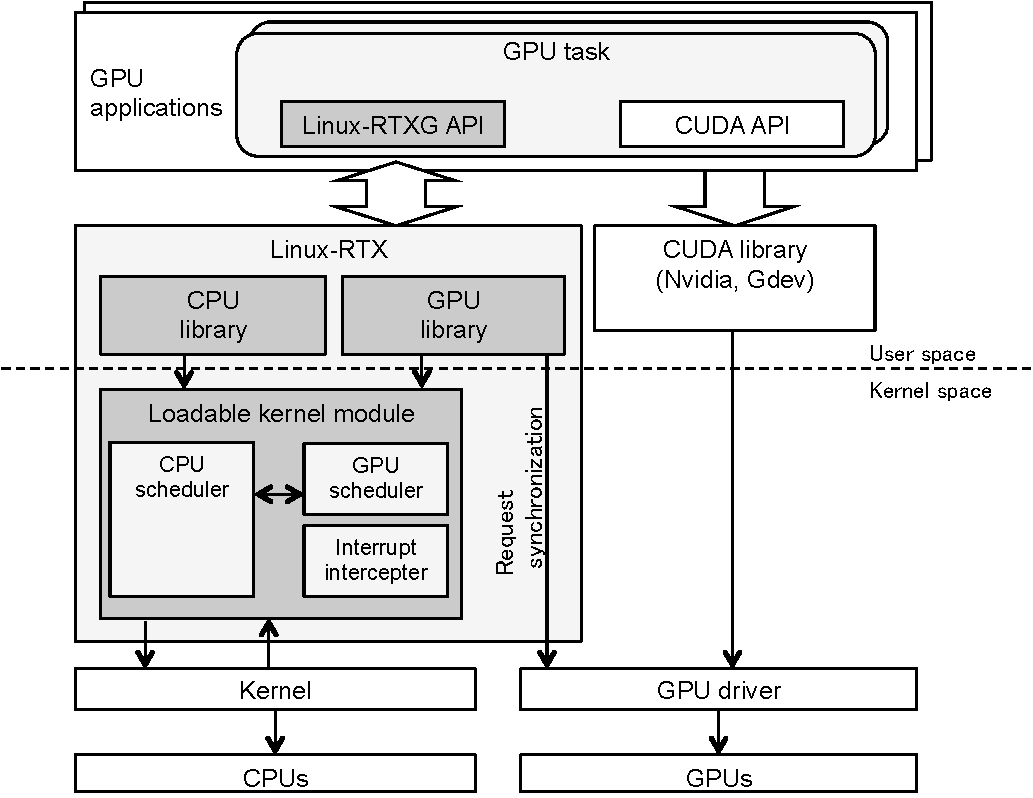
\includegraphics[width=0.35\textwidth]{img/overview.pdf}
\caption{Over view of the Linux-RTXG}
\end{center}
\label{fig:overview}
\end{figure}

Figure~\ref{fig:overview} shows over-view of linux-rtxg.
Linux-rtxg is divided into two components that are loadable kernel module and library.
linux-rtxg library is interface of communicate between application and linux-rtxg core component(kernel module).
it is using system call that is ioctl.

The part of library included speciall method that is independent synchronization method.
it method is used only on the nvidia driver.
if system use nouveau driver, runtime must use part of gdev.
Gdev can happen arbitary interrupt of gpu kernel in the user-space mode, and it have no need to be independent interrupt raised method.

linux-rtxg loadable kernel module is positioned kernel-space.
Thus, module can use kernel exported function.

\subsection{GPU Scheduler}
\begin{table*}[t]
\begin{center}
\caption{Basic Linux-RTXg APIs}
\label{tab:rtx-api}
\begin{tabular}{|l|p{50em}|} \hline
rtx\_gpu\_open() & To register itself to linux-RTXg, and create scheduling entity. It will must call first. \\ \hline
rtx\_gpu\_device\_advice() & To get the recommendation of GPU devices to be used \\ \hline
rtx\_gpu\_launch() & To control the GPU kernel launch timing, in other words it is scheduling entry point. It will must call before the CUDA launch API. \\ \hline
rtx\_gpu\_sync() & To wait for finishing GPU kernel execution by sleeping with TASK UNINTERRUPTIBLE status.\\ \hline
rtx\_gpu\_notify() & To register the notify/fence command to GPU microcontroller. The fence or the notify is selected flag is set by argument.\\ \hline
rtx\_gpu\_close() & To release scheduling entity.\\ \hline
\end{tabular}
\end{center}
\end{table*}

Linux-RTXg's scheduler function is provided RTXG API.
The basic APIs supported by Linux-RTXg are listed in Table~\ref{tab:rtx-api}.
Some APIs have arguments and others do not.
Our API is not modificated existing CUDA API to cope with proprietary software to be independent from the runtime.
However, user have to add linux-rtxg api to existing CUDA application for using linux-rtxg scheduler.

\begin{figure}[t]
\begin{center}
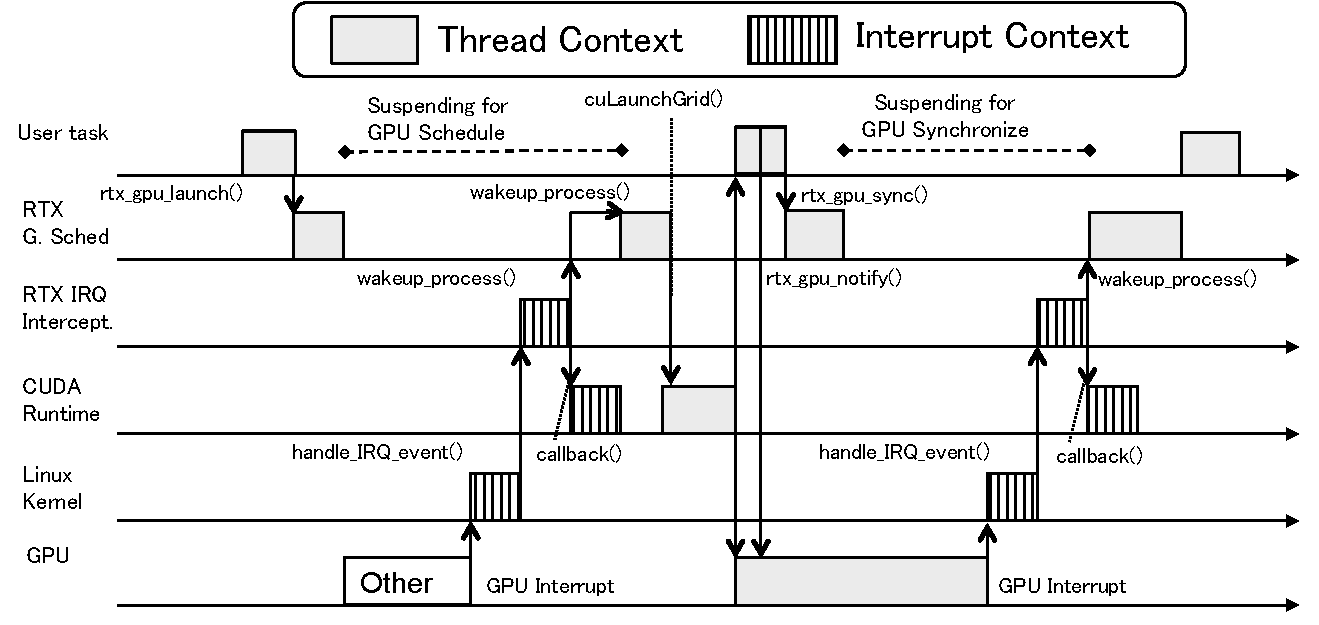
\includegraphics[width=0.5\textwidth]{img/gsched_controlflow.pdf}
\caption{GPU Scheduling control flow}
\end{center}
\label{fig:controlflow}
\end{figure}

Figure~\ref{fig:controlflow} shows control flow of the wakeup GPU job on the linux-rtxg's gpu scheduler.
The configure is GPUカーネルの発行はひとつに制限されており、すでにGPUでタスクがうごいている状態とし、同期は割込みを用いたNOTIFYによって行うものとする。
ユーザタスクは$rtx_gpu_launch()$を呼び出すことで、GPUカーネル実行のタイミングをコントロールすることができる。
設定通り、既にGPUでタスクが動いており、現在カーネル発行を許可されているタスクが自身でないため、割込みによって起床されるまでtask uninterruptible状態で自らスリープに入る。
動いていたタスクが終了した時点で割込みが発行され、そのコンテキストのInterrupt intercepterによってスリープしていた次のタスクが起床される。

起床したタスクは$cuLaunchGrid()$などのCUDA APIを通じてGPUカーネルの発行を行う。
カーネル発行後、割込みを発生させるためのNotifyの登録を行い、その割込みが発生するまでスリープに入る。

割込みが発生すると次のタスクが動作するといったフローを持ってスケジューリングが行われる。
次のタスクの選択は、割込みによって起こされるGPU schedulerによって行われる。

\subsection{GPU synchronization}
本スケジューラsynchronization basedなスケジューラでありGPUカーネルのラウンチを要求されたタイミングと、そのカーネルが終了したタイミングを知る必要がある。
Linux-RTXGでは前述のようにrtx\_gpu\_launch()によってGPUカーネルのラウンチ要求を受け取る.
アプリケーションはrtx\_gpu\_launch()を呼び出すことでioctlシステムコールによって、ユーザコンテキストからカーネルコンテキストへと処理が移り、スケジューラが保持するGPUタスク情報 (e.g. waiting task status, running task status, GPU device status) を基に自身が動作可能かを確認し動作する。スケジューラを通じて、資源を獲得できた場合にはGPUカーネルのラウンチの発行が可能となる。

ラウンチされたカーネルが終了したタイミングをスケジューラはNOTIFYかFENCEによって取得する。
NOTIFYかFENCEはNVIDIAのプロプライエタリ・ソフトウェアではコンテキスト生成時にフラグをセットすることで発生させることが可能であるが、どのカーネルが終了したかの識別と、
rtx\_gpu\_notify()、もしくはランタイムによって発生される割込みを獲得するか、cuCtxSynchronize後にrtx\_gpu\_sync()に専用フラグをセットすることで呼び出す

\textbf{Interrupt interception:}
割込みはデバイスドライバ(カーネルと共にパッケージされている)によって登録されたISRがハンドルする。

Linux-RTXGではタスクの選択のためにワーカースレッドを保持する。
本ワーカースレッドは実行中のカーネルが終了した時点で次のタスクの選択を行う。
ワーカースレッドはタスクの選択後にCPU資源を他のタスクに明け渡すためにサスペンドに入る。
これらを適切に立ち上げるためには任意の割込みを獲得し、外部ISRがその割込みがどのカーネルに関連しているかを識別できる仕組みが必要である。加えて、割込みの識別はGPUのステータス・レジスタを読み込んで行う必要があり、GPUドライバが割込みレジスタをリセットする前に、実行される必要がある。

Linuxでは、割込み番号ごとにirq\_descという割込みのパラメータを保持する構造体を持っている。
この構造体にはISRの関数ポインタを含むirq\_actionという構造体がリストで接続されている。
irq\_descはグローバルな領域に確保されており、カーネル空間からであれば誰でも参照可能である。
Linuxのローダブルカーネルモジュールはカーネル空間で動作しているため、このirq\_descを取得でき、
Interrupt handlerの関数ポインタも取得可能である。

我々はこの取得した関数ポインタを保持し、我々の傍受用ISRをカーネルに登録する。
そして傍受用ISRで、事前に保持しておいたGPUドライバの割込みハンドラの関数コールバック関数として呼び出すことで、通常の割込みハンドリングを実行する。
加えて我々のこれまでの研究\cite{fujii:icpads2013,kato2013zero}で、GPUのio registerはPCIeのBAR0によって指定されたアドレスから存在しておりカーネル空間にデバイスドライバによってマッピングされていることがわかっている。
そのためLinux-RTXGが傍受用ISRの初期化の際に$ioremap()$によってBAR0空間をマッピングしておき、傍受用ISRが呼び出された際にマッピングされたレジスタを読み込むことで、
割込みの識別を行う。


\textbf{Independent generate sign for Synchronization:}
ここでは、ランタイムから独立した割込み機構として、独自にNOTIFY、FENCEに用いるsignを発生させる仕組みを提供する。
ここでのsignは、NOTIFYは割込み、FENCEはmappedメモリへの値の書き込みである。
NVIDIAのクローズドソースドライバはNouveauプロジェクトのリバースエンジニアリングによる解析によって、ioctlを使ったインタフェースになっていることがわかっている。
Gdevではこの解析された情報を用いて、NVIDIAのクローズドソースドライバとオープンソースライブラリという掛け合わせでCUDAを実行できる基盤が構築されている。
本論文では、この基盤から割込みを発生させる部位のみ抽出し、スケジューリングに用いる。

本メソッドは大きく2つに分かれ、それぞれInitializeとNotifyと呼ぶ。
Initializeは、いわゆるコンテキストの生成に値する。Virtual Address Spaceやコマンド送信に用いるIndirect Bufferの確保、コンテキストオブジェクトの生成などを行う。
NotifyはComputeエンジンやCopyエンジンに向けて割込み発生、もしくはFENCE用に値の書き込みを行うコマンドを送信する。

本アプローチに用いるインタフェースは公式にサポートされていないために、ベンダーによる急な仕様変更には対応できない。
しかしながら、これ以外に割込みを発生させるアプローチがなく、クローズドソースを用いた場合の限界であるといえる。

\subsection{Scheduler Integration}
Linux scheduler have various real-time scheduling policies that were SCHED\_DEADLINE, SCHED\_FIFO and SCHED\_RR.
特にSCHED\_DEADLINEはLinux 3.14よりメインラインに含まれたConstant Bandwidth ServerとGlobal-EDFの実装であり、
Linuxをリアルタイム拡張するにおいて有効に利用できるクラスである。
However, synchronization does not work well in a SCHED\_DEADLINE scheduling policy when using GPU tasks.

本問題は2種類存在しており、
sched\_yield()によるCPU放棄の実装によるものと、
suspendingした後の復帰の実装によるものである。

一つ目のsched\_yield(カーネル内ではyield関数)は、FENCEのようにPollingされる場合に生じる。
pollingはCPUを専有してしまう方式であり、他のタスクへの影響を考えた場合、一度CPUを放棄したほうが良い結果が得られる場合がある。
しかしながらsched\_yieldでは、SCHED\_DEADLINEの内部パラメータとして扱う、runtime(残りの実行しても良い時間)を0にしてしまう。
これによって、次の周期が訪れるまではruntimeが補充されることがなく、そのタスクは実行権限を失う。
sched\_yieldはGPUランタイムに限らず、デバイスドライバやライブラリなどで多く利用されており、
それら全てで、SCHED\_DEADLINEポリシー上では正常に動作しない結果が生じる可能性が高い。
NVIDIAのCUDAにおいても同期フラグの設定次第で本問題に影響を受ける。
Linux-RTXGではSCHED\_DEADLINE時はNOTIFYを使うことを推奨し、sched\_yieldの利用を制限することで対応した。

2つ目の問題はタスクが一度sleeping状態に入り、復帰時に式(1)を用いて実行可能性についてチェックを行う。
式(1)が真の時、runtimeが補充され、absolute deadlineが次の周期に設定される。

{\scriptsize
\begin{equation}
\frac{Absolute\_Deadline - Current\_Time}{Remaining\_Runtime} > \frac{Relative\_Deadline}{Period}
\end{equation}
}

linux-rtxgでは本チェックについて、sleeping状態から起床するという状態を、
GPUカーネル実行による復帰と、周期による復帰とで種類分けし、
GPUカーネル実行による復帰時にのみ、$Remaining\_Runtime$からGPU execution timeを引くことで対応した。

